\section{Simulated data}
\subsection{Classification}

All results should be reported with k-fold cross validation accuracies, using
standard deviation in the folds as an uncertainty estimate.
\begin{itemize}
  \item ? - Logistic regression results to argue necessity for more complex model
  \item ? - Dense network to demonstrate increased performance over logistic
  \item ? - Pretrained network? VGG since we base the architecture of current model on the VGG paper recommendations?
  \item Project model - Attempt to reproduce results. k-fold results on same data as current model
  \item Current best performing model for classifications
\end{itemize}

\begin{figure}
\centering
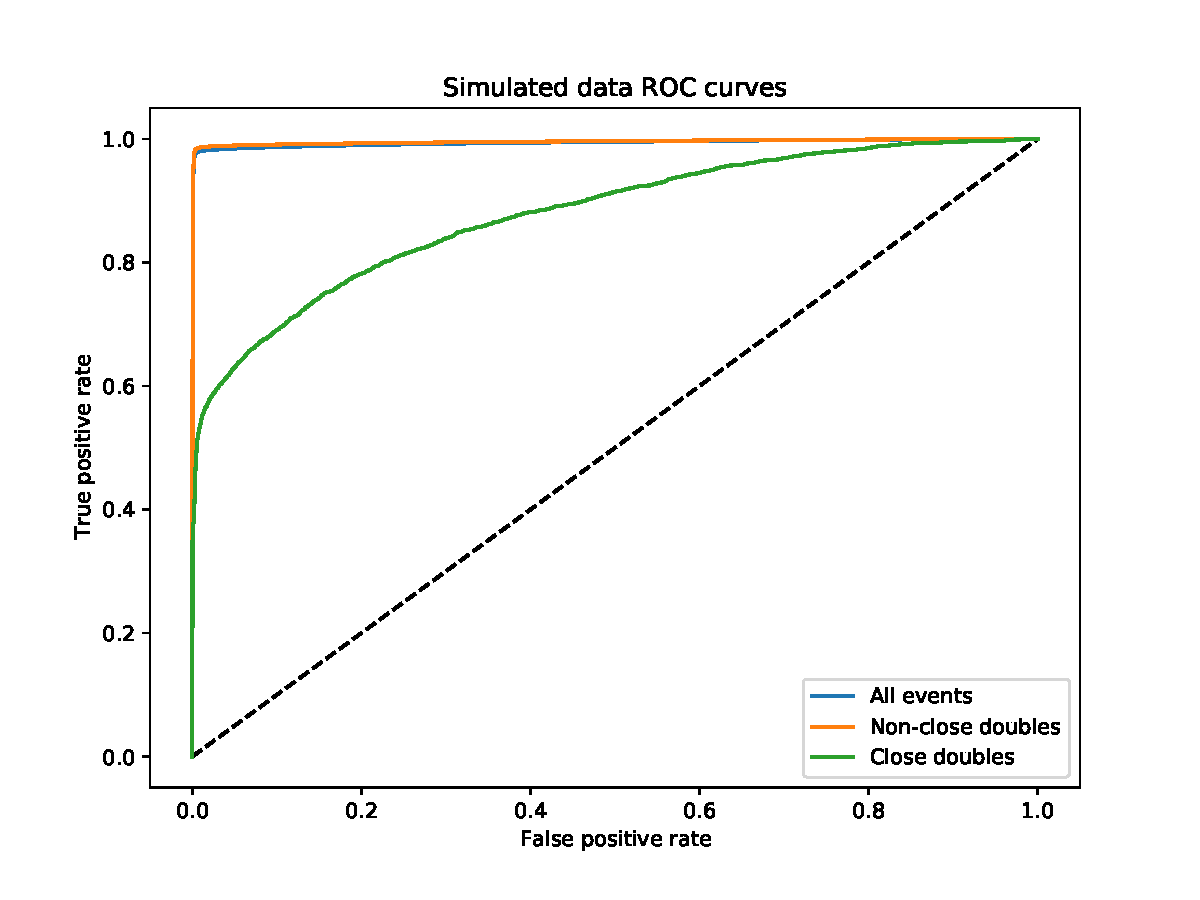
\includegraphics[width=0.8    \textwidth, height=6.5cm]{chapters/results/figures/roc_simulated.pdf}
\caption[Titletext]{generic text}\label{fig:roc_simulated}
\end{figure}

\subsection{Regression}
Same approach as for classification.
\begin{itemize}
  \item ? - Linear approach?
  \item ? - Dense network                                                                   Q
  \item ? - CNN
\end{itemize}
\subsubsection{Position}
\subsubsection{Energy}
\subsection{Experimental data}
\subsection{Classification}
\subsection{Regression}
\subsubsection{Position}
\subsubsection{Energy}
